\section{Transfert Du Fichier Malveillant}

\begin{center}
    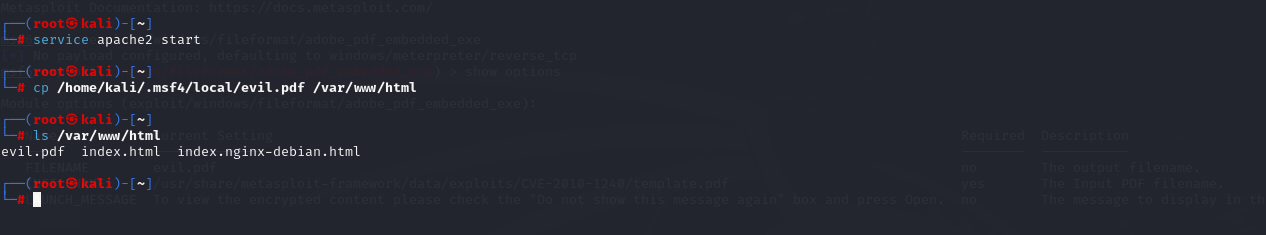
\includegraphics[width=0.8\textwidth]{Question/SC/9_10_11-.PNG}
\end{center}

\vspace{0.15cm}

\begin{center}
    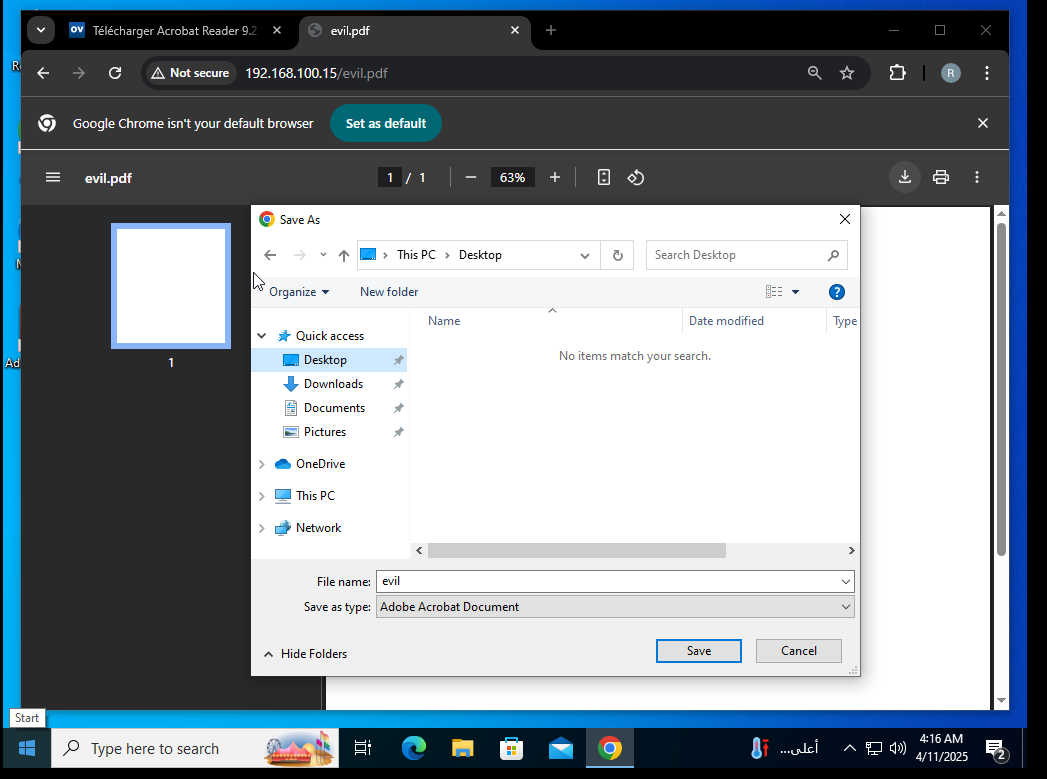
\includegraphics[width=0.6\textwidth]{Question/SC/12_1-.PNG}
\end{center}

\vspace{0.15cm}

\begin{center}
    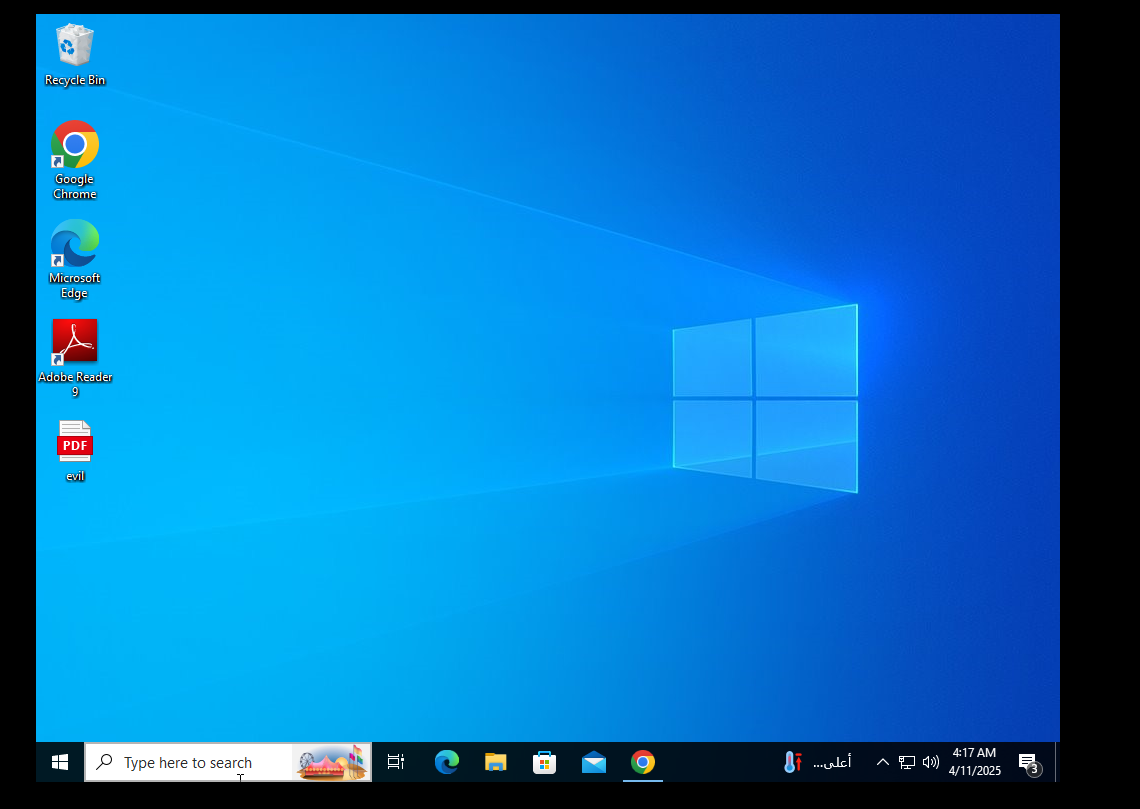
\includegraphics[width=0.6\textwidth]{Question/SC/12_2.PNG}
\end{center}


\vspace{0.35cm}

\begin{prettyBox}{Transfert de fichiers malveillants}{myblue}
\begin{itemize}
    \item On peut transférer le fichier à l'utilisateur sous un nom différent par email, lien, programme qui force l'installation, etc.
    \item La commande \texttt{cp <path> /var/www/html} met une copie du fichier dans le répertoire /var/www/html qui représente le chemin des fichiers du serveur Apache
\end{itemize}
\end{prettyBox}
